\documentclass[conference]{IEEEtran}
\IEEEoverridecommandlockouts
\usepackage{cite}
\usepackage{amsmath,amssymb,amsfonts}
\usepackage{algorithmic}
\usepackage{graphicx}
\usepackage{textcomp}
\usepackage{xcolor}
\usepackage{tikz}
\usetikzlibrary{shapes,arrows,positioning,fit,calc}

\def\BibTeX{{\rm B\kern-.05em{\sc i\kern-.025em b}\kern-.08em
    T\kern-.1667em\lower.7ex\hbox{E}\kern-.125emX}}

\begin{document}

\title{Contextual Product Recommender Platform Based on User Digital Activity Patterns}

\author{\IEEEauthorblockN{Vignesh}
\IEEEauthorblockA{\textit{Department of Master of Computer Applications} \\
\textit{Ramaiah Institute of Technology}\\
Bengaluru, India}
\and
\IEEEauthorblockN{Dr. Preethi N Patil}
\IEEEauthorblockA{\textit{Associate Professor} \\
\textit{Department of Master of Computer Applications} \\
\textit{Ramaiah Institute of Technology}\\
Bengaluru, India}
}

\maketitle

\begin{abstract}
The rapid expansion of user interactions across heterogeneous digital channels has introduced significant challenges for contemporary recommendation systems, particularly in maintaining unified user identities and delivering relevant, context-aware recommendations. User activity data generated from web applications, mobile platforms and external digital services is often stored in isolated silos, resulting in fragmented user profiles and inconsistent personalization outcomes. This fragmentation limits the system's ability to accurately capture evolving user interests and frequently leads to repetitive or irrelevant recommendations. This work proposes a Contextual Product Recommender Platform that addresses these challenges through a unified and adaptive system architecture. The platform supports the ingestion of high-speed interaction streams in real-time using Apache Kafka, enabling a timely analysis of user behavior. An identity resolution mechanism is used to consolidate distributed interaction signals across multiple channels into a single unified user representation, referred to as a User Node. This unified profile enables holistic cross-channel behavior analysis and dynamic interest modeling. The recommendation engine is built upon content-based filtering techniques and continuously updates user interest scores based on recent behavioral signals, including clicks, ignores and dismissals. To reduce recommendation fatigue, the system incorporates adaptive suppression logic that filters redundant or low-relevance items based on user feedback and temporal constraints. Overall, the proposed platform enhances recommendation relevance, improves adaptability to changing user preferences and supports scalable deployment in multi-channel digital environments.
\end{abstract}

\begin{IEEEkeywords}
Recommendation Systems, Identity Resolution, User Behavior, Context Awareness
\end{IEEEkeywords}

\section{Introduction}
The rapid growth of digital platforms has significantly transformed the way users interact with online systems, resulting in the generation of large volumes of behavioral data across web applications, mobile platforms and other digital channels. These interaction signals, which include clicks, page views, browsing duration and feedback actions, provide valuable insights into user preferences and intent. However, in many real-world systems, such data is collected and stored in isolated data silos, leading to fragmented user representations and limiting the effectiveness of personalized recommendation delivery.

Traditional recommendation systems often rely on historical interaction data or static user profiles, assuming relatively stable user interests. As user behavior evolves rapidly across multiple channels, such assumptions frequently result in outdated, repetitive, or irrelevant recommendations, thereby reducing user engagement and trust in the system. Furthermore, the lack of real-time behavioral analysis and cross-channel identity integration prevents systems from adapting promptly to changes in user intent.

To address these challenges, this work proposes a Contextual Product Recommender Platform that processes real-time user interactions, including clicks, page views and dismissal events, to generate adaptive and context-aware recommendations. By integrating real-time data ingestion, unified user profiling and dynamic interest modeling, the proposed platform aims to enhance recommendation relevance, reduce redundancy and improve overall user experience in multi-channel digital environments.

\section{Literature Review}
Recommendation systems have been extensively studied to enhance personalization by analyzing user interaction data and behavioral patterns. Early research in adaptive personalization demonstrated that interaction signals such as navigation paths, dwell time and click behavior can be used to dynamically tailor system content \cite{kumar2024adaptive}. Techniques including clustering algorithms such as K-means and BIRCH group users based on behavioral similarity rather than static demographic attributes, leading to improved personalization accuracy. However, these approaches are typically limited to single-platform environments and do not address identity fragmentation across multiple digital channels.

Content-based filtering methods are widely adopted in media, e-commerce and information systems, where item attributes such as keywords, genres and metadata are matched with user preferences \cite{sahu2022movie}. While effective in domains with rich metadata, these systems rely heavily on historical interaction data and assume relatively stable user interests. As a result, they often struggle to adapt to rapid changes in user behavior and may generate repetitive or outdated recommendations. Similar limitations are observed in domain-specific recommendation systems, such as smart library platforms \cite{liu2024design}, which improve relevance but lack support for real-time feedback integration and cross-platform identity resolution.

Context-aware recommender systems extend traditional models by incorporating contextual information such as time, location, device type and session context to improve situational relevance \cite{adomavicius2005context}. Although these approaches enhance recommendation quality, most implementations assume consistent user identities and fail to address fragmented behavioral signals generated across heterogeneous channels. Advanced techniques such as cross-domain \cite{li2023cdrec} and personality-aware \cite{dhelim2021personality} recommendation systems attempt to mitigate cold-start and sparsity issues but are generally complex, computationally intensive and evaluated in offline settings. Furthermore, models like Markov-based prediction \cite{awad2012prediction} help anticipate short-term goals but lack long-term cross-channel state.

In summary, existing literature primarily focuses on algorithm-level improvements and batch-based evaluation, with limited emphasis on real-time data ingestion, unified user identity management, adaptive feedback handling and scalable system architectures.

\sectionsection{Problem Definition and Objectives}
The rapid growth of digital platforms has resulted in user interaction data being generated across multiple channels, often leading to fragmented user identities and incomplete behavioral understanding. Existing recommendation systems struggle to unify these distributed signals, which limits their ability to construct accurate user profiles and deliver relevant recommendations. There is a need for a unified platform that consolidates user identities, builds dynamic user profiles and continuously refines recommendations by learning from real-time user feedback.

The objectives of the proposed system are as follows:
\begin{itemize}
    \item To ingest user interaction data shared by partnered digital platforms and unify it into a single dataset by resolving user identities across multiple channels.
    \item To develop dynamic global user profiles by analyzing contextual signals, historical behavior, and evolving interest patterns.
    \item To implement a personalized recommendation mechanism based on content-based filtering that adapts in real time by learning from both positive feedback signals and negative feedback signals.
\end{itemize}

\section{Proposed Methodology}
The proposed methodology aims to address the limitations identified in existing recommendation systems by introducing a unified, real-time and adaptive recommendation framework. The methodology is designed to process high-velocity user interaction data, resolve fragmented user identities, and dynamically generate personalized recommendations based on evolving behavioral patterns.

User interaction data, including clicks, page views, browsing duration, ignores and dismissals, is continuously collected from multiple digital channels. These interaction events are ingested in real time using a streaming infrastructure, enabling low-latency processing and timely behavioral analysis. To overcome identity fragmentation, an identity resolution mechanism consolidates interaction signals originating from different platforms and devices into a single unified user representation. This unified profile captures cross-channel behavior and forms the basis for accurate personalization.

Based on the unified user profile, dynamic interest modeling is performed by updating interest scores according to recent behavioral signals. A content-based filtering approach is employed to match product attributes with the user's current interests, ensuring that recommendations remain aligned with evolving preferences. Unlike static recommendation models, the proposed methodology continuously adapts to changes in user behavior.

To minimize recommendation redundancy and user fatigue, an adaptive suppression mechanism is integrated into the recommendation pipeline. This mechanism leverages negative feedback signals and temporal constraints to suppress low-relevance or previously dismissed items for a defined duration. By combining real-time data ingestion, unified identity resolution, adaptive interest modeling and intelligent suppression logic, the proposed methodology delivers context-aware, non-redundant and personalized recommendations suitable for multi-channel digital environments.

\section{System Design}
The system is designed using a modular client--server architecture to support real-time processing of user interactions and scalable recommendation delivery. External digital applications act as clients that communicate with the recommendation platform through secure RESTful APIs. These APIs handle interaction data submission and recommendation requests while ensuring controlled and authenticated access.

At the core of the system design is the data ingestion layer, which captures user interaction events such as clicks, page views, ignores and dismissals from multiple digital channels. These events are streamed in real time to the processing layer, enabling timely behavioral analysis. The processing layer is responsible for identity resolution, interest modeling and recommendation generation.

\begin{figure}[htbp]
\centerline{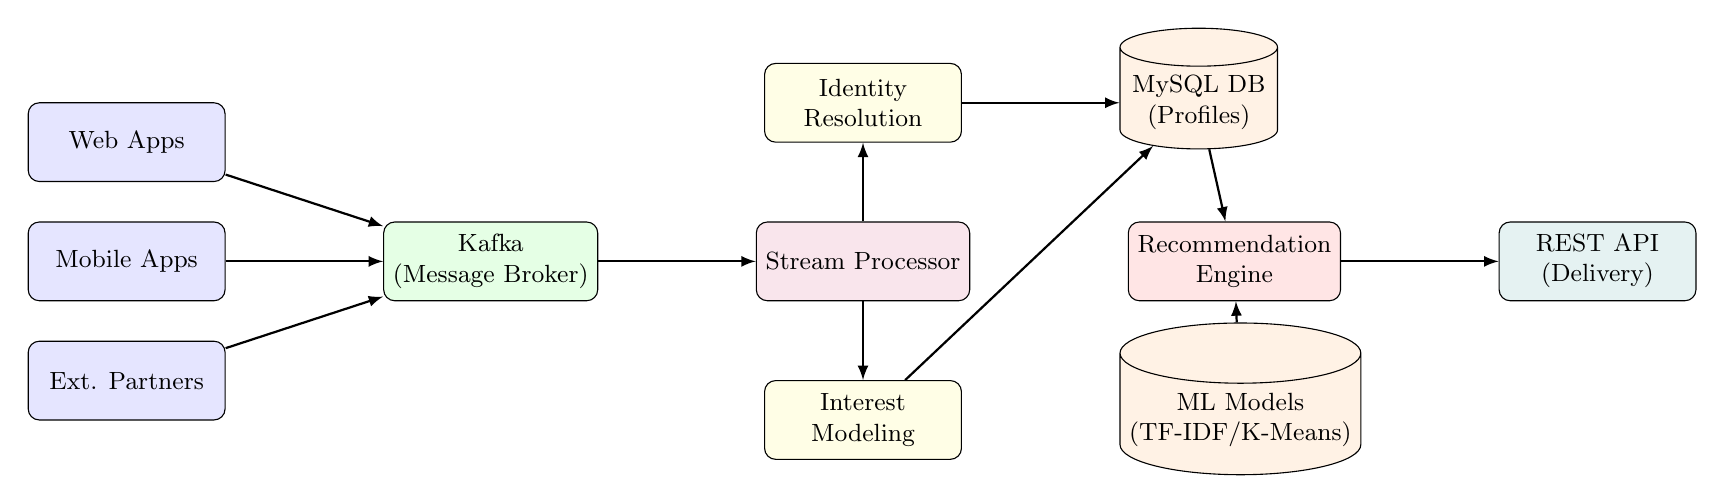
\begin{tikzpicture}[
    node distance=1.5cm and 2cm,
    box/.style={rectangle, draw, rounded corners, align=center, fill=blue!10, minimum width=2.5cm, minimum height=1cm, font=\small},
    db/.style={cylinder, draw, shape border rotate=90, aspect=0.25, align=center, fill=orange!10, minimum width=2cm, minimum height=1.5cm, font=\small},
    arrow/.style={-latex, thick}
]

% Nodes
\node[box] (web) {Web Apps};
\node[box, below=0.5cm of web] (mobile) {Mobile Apps};
\node[box, below=0.5cm of mobile] (external) {Ext. Partners};

\node[box, right=2cm of mobile, fill=green!10] (kafka) {Kafka \\ (Message Broker)};

\node[box, right=2cm of kafka, fill=purple!10] (stream) {Stream Processor};

\node[box, above=1cm of stream, fill=yellow!10] (id_res) {Identity \\ Resolution};
\node[box, below=1cm of stream, fill=yellow!10] (interest) {Interest \\ Modeling};

\node[db, right=2cm of id_res] (mysql) {MySQL DB \\ (Profiles)};
\node[db, right=2cm of interest] (model_db) {ML Models \\ (TF-IDF/K-Means)};

\node[box, right=2cm of stream, fill=red!10] (rec_engine) {Recommendation \\ Engine};

\node[box, right=2cm of rec_engine, fill=teal!10] (api) {REST API \\ (Delivery)};

% Edges
\draw[arrow] (web) -- (kafka);
\draw[arrow] (mobile) -- (kafka);
\draw[arrow] (external) -- (kafka);

\draw[arrow] (kafka) -- (stream);

\draw[arrow] (stream) -- (id_res);
\draw[arrow] (stream) -- (interest);

\draw[arrow] (id_res) -- (mysql);
\draw[arrow] (interest) -- (mysql);

\draw[arrow] (mysql) -- (rec_engine);
\draw[arrow] (model_db) -- (rec_engine);

\draw[arrow] (rec_engine) -- (api);

\end{tikzpicture}
}
\caption{System Architecture of CPRP}
\label{fig:arch}
\end{figure}

The identity resolution component plays a critical role in unifying fragmented user interactions. It matches multiple identifiers, such as email addresses and phone numbers, to construct a single consolidated user profile. This unified profile enables cross-channel behavior analysis and forms the foundation for accurate personalization.

\begin{figure}[htbp]
\centerline{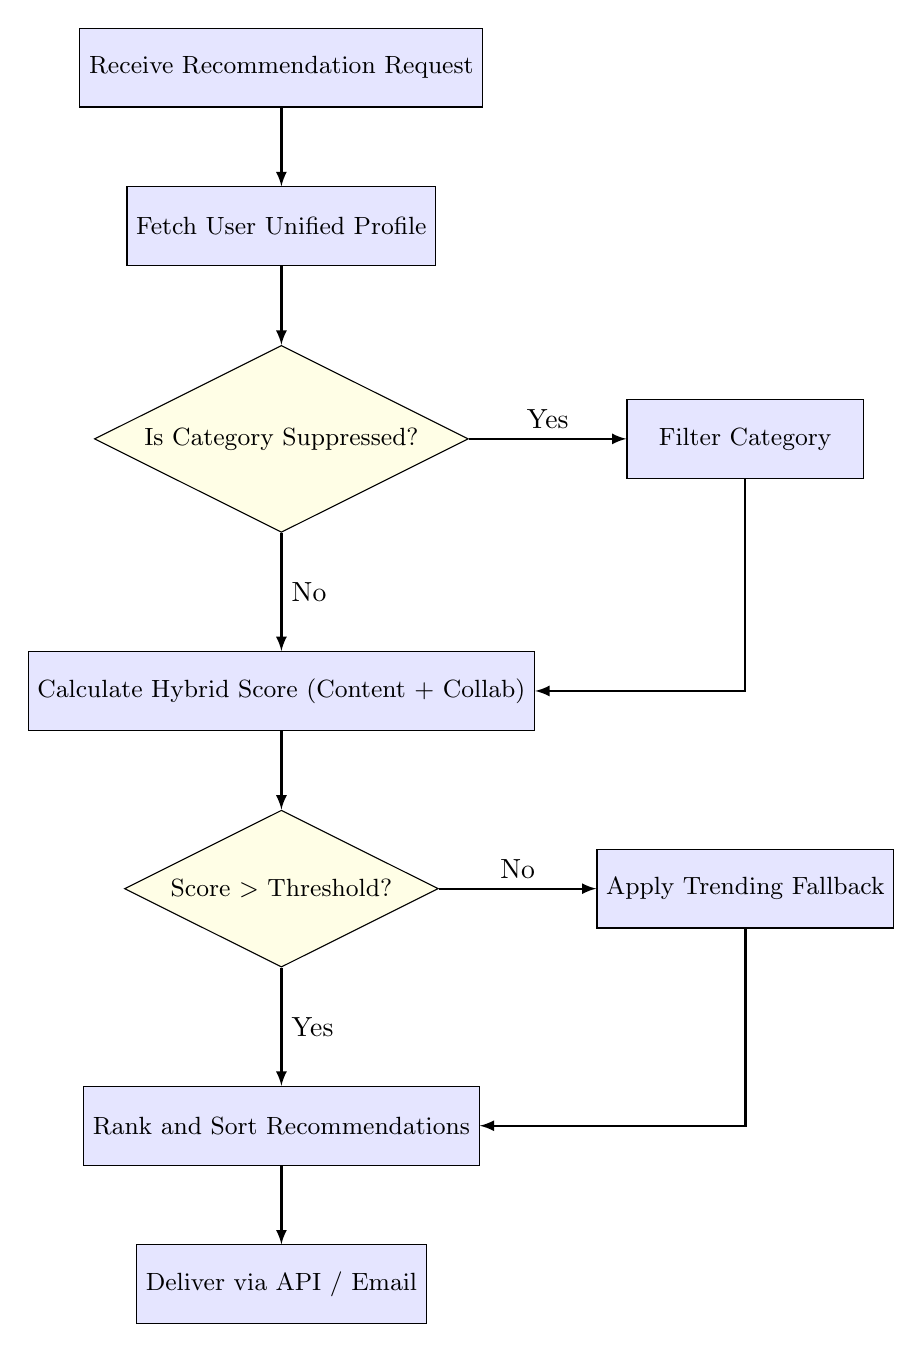
\begin{tikzpicture}[
    node distance=1.5cm and 2cm,
    process/.style={rectangle, draw, align=center, fill=blue!10, minimum width=3cm, minimum height=1cm, font=\small},
    decision/.style={diamond, draw, align=center, fill=yellow!10, aspect=2, font=\small},
    arrow/.style={-latex, thick}
]

% Nodes
\node[process] (start) {Receive Recommendation Request};
\node[process, below=1cm of start] (fetch_profile) {Fetch User Unified Profile};
\node[decision, below=1cm of fetch_profile] (is_suppressed) {Is Category Suppressed?};
\node[process, right=2cm of is_suppressed] (skip) {Filter Category};
\node[process, below=1.5cm of is_suppressed] (calc_score) {Calculate Hybrid Score (Content + Collab)};
\node[decision, below=1cm of calc_score] (above_threshold) {Score $>$ Threshold?};
\node[process, right=2cm of above_threshold] (fallback) {Apply Trending Fallback};
\node[process, below=1.5cm of above_threshold] (sort) {Rank and Sort Recommendations};
\node[process, below=1cm of sort] (end) {Deliver via API / Email};

% Edges
\draw[arrow] (start) -- (fetch_profile);
\draw[arrow] (fetch_profile) -- (is_suppressed);

\draw[arrow] (is_suppressed) -- node[above] {Yes} (skip);
\draw[arrow] (is_suppressed) -- node[right] {No} (calc_score);

\draw[arrow] (skip) |- (calc_score);

\draw[arrow] (calc_score) -- (above_threshold);

\draw[arrow] (above_threshold) -- node[above] {No} (fallback);
\draw[arrow] (above_threshold) -- node[right] {Yes} (sort);

\draw[arrow] (fallback) |- (sort);

\draw[arrow] (sort) -- (end);

\end{tikzpicture}
}
\caption{Recommendation Flow Diagram}
\label{fig:flow}
\end{figure}

Based on the unified user profile, the recommendation engine applies content-based filtering techniques to match product attributes with dynamically updated user interests. To enhance recommendation quality, an adaptive suppression mechanism is integrated into the design. This mechanism analyzes user disinterest signals and temporal constraints to suppress redundant or low-relevance items, thereby reducing recommendation fatigue.

\begin{figure}[htbp]
\centerline{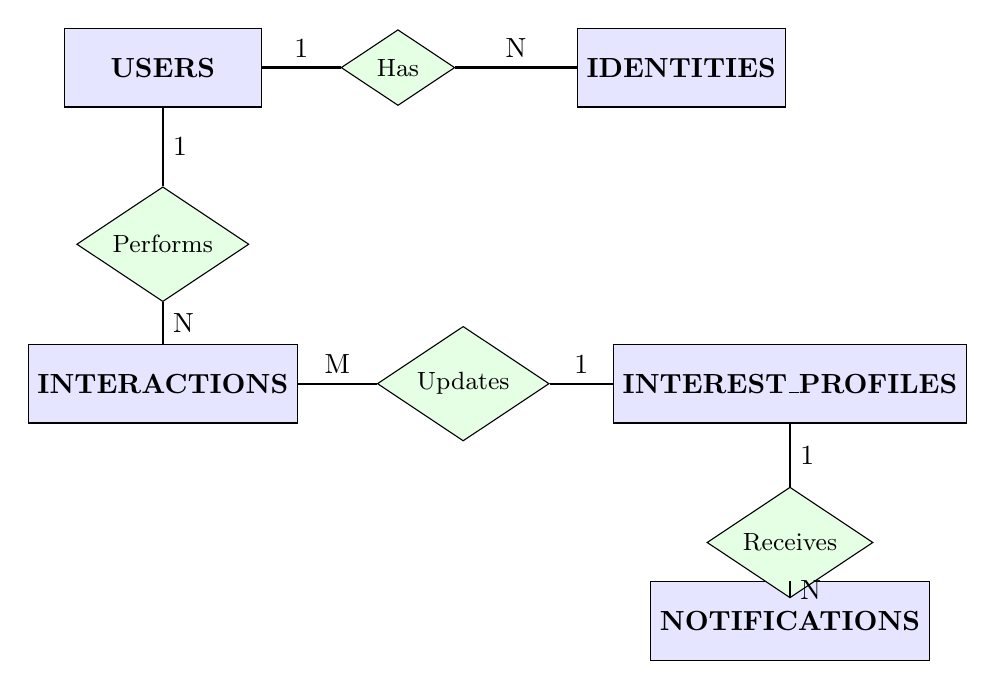
\begin{tikzpicture}[
    node distance=2cm and 2cm,
    entity/.style={rectangle, draw, align=center, fill=blue!10, minimum width=2.5cm, minimum height=1cm, font=\bfseries},
    attr/.style={ellipse, draw, align=center, fill=yellow!10, minimum width=2cm, font=\small},
    rel/.style={diamond, draw, align=center, fill=green!10, aspect=1.5, font=\small},
    line/.style={thick}
]

% Entities
\node[entity] (users) {USERS};
\node[entity, right=4cm of users] (identities) {IDENTITIES};
\node[entity, below=3cm of users] (interactions) {INTERACTIONS};
\node[entity, right=4cm of interactions] (profiles) {INTEREST\_PROFILES};
\node[entity, below=2cm of profiles] (notifications) {NOTIFICATIONS};

% Relationships
\node[rel, right=1cm of users] (has_id) {Has};
\node[rel, below=1cm of users] (performs) {Performs};
\node[rel, right=1cm of interactions] (updates) {Updates};
\node[rel, below=0.8cm of profiles] (receives) {Receives};

% Lines connecting Entities to Relationships
\draw[line] (users) -- (has_id) node[midway, above] {1};
\draw[line] (has_id) -- (identities) node[midway, above] {N};

\draw[line] (users) -- (performs) node[midway, right] {1};
\draw[line] (performs) -- (interactions) node[midway, right] {N};

\draw[line] (interactions) -- (updates) node[midway, above] {M};
\draw[line] (updates) -- (profiles) node[midway, above] {1};

\draw[line] (profiles) -- (receives) node[midway, right] {1};
\draw[line] (receives) -- (notifications) node[midway, right] {N};

\end{tikzpicture}
}
\caption{Database Entity-Relationship Diagram}
\label{fig:er}
\end{figure}

The system is implemented using Python for data processing and model execution, Flask for API services, Scikit-learn for recommendation logic and Docker for containerized deployment. This modular system design improves scalability, maintainability and ease of integration with external platforms.

\section{Future Enhancements}
The proposed platform is designed with extensibility in mind, allowing several enhancements to be incorporated in future iterations. One possible enhancement is the integration of hybrid recommendation techniques that combine content-based filtering with collaborative filtering to improve recommendation diversity and accuracy. Incorporating advanced machine learning models such as deep learning-based representation learning can further enhance interest modeling for complex user behavior patterns.

Future versions of the system can also support multi-domain recommendation by leveraging cross-domain behavioral signals to reduce cold-start challenges. The inclusion of richer contextual signals such as location data, device usage patterns and temporal trends can further improve recommendation relevance. Additionally, real-time analytics dashboards may be introduced to provide administrators with deeper insights into system behavior and user engagement trends.

From an architectural perspective, the platform can be extended to support large-scale deployment using distributed data stores and cloud-native orchestration tools. Enhancing privacy-preserving mechanisms through anonymization techniques and compliance-aware data handling strategies can further strengthen trust and regulatory alignment. These enhancements will improve scalability, adaptability and robustness of the recommendation platform in evolving digital environments.

\section{Conclusion}
This paper presented the design and documentation of a Contextual Product Recommender Platform based on user digital activity patterns. The proposed system addresses key challenges associated with fragmented user identities, static user profiling and repetitive recommendation delivery in multi-channel digital environments. By emphasizing unified identity resolution, real-time interaction processing and adaptive recommendation logic, the platform provides a structured foundation for delivering personalized and context-aware recommendations.

The documentation detailed the system architecture, design principles and methodology required to build a scalable and modular recommendation platform. The inclusion of adaptive suppression mechanisms ensures reduction of recommendation fatigue while maintaining relevance. Although the current work focuses on system design and documentation, it establishes a strong groundwork for future implementation and evaluation.

Overall, the proposed platform demonstrates the feasibility of integrating real-time data ingestion, unified user profiling and adaptive personalization within a single framework. This work serves as a foundation for further development toward a fully implemented and production-ready recommendation system capable of supporting modern multi-channel digital platforms.

\bibliographystyle{IEEEtran}
\bibliography{references}

\end{document}
